\documentclass[letterpaper,11pt]{article}
\usepackage[left=1.4cm,right=1.4cm,top=1.5cm, bottom=1.5cm]{geometry}
\usepackage{mathpazo}
\usepackage{graphicx,color}
\usepackage[colorlinks=true, urlcolor=blue, linkcolor=blue, citecolor=blue]{hyperref}
\usepackage{enumitem}

\setlist[description]{noitemsep, topsep=2pt}

\pagestyle{empty}

\begin{document}

% --- Header with photo ---
\noindent
\begin{minipage}[t]{0.22\textwidth}
    \vspace{0pt}
    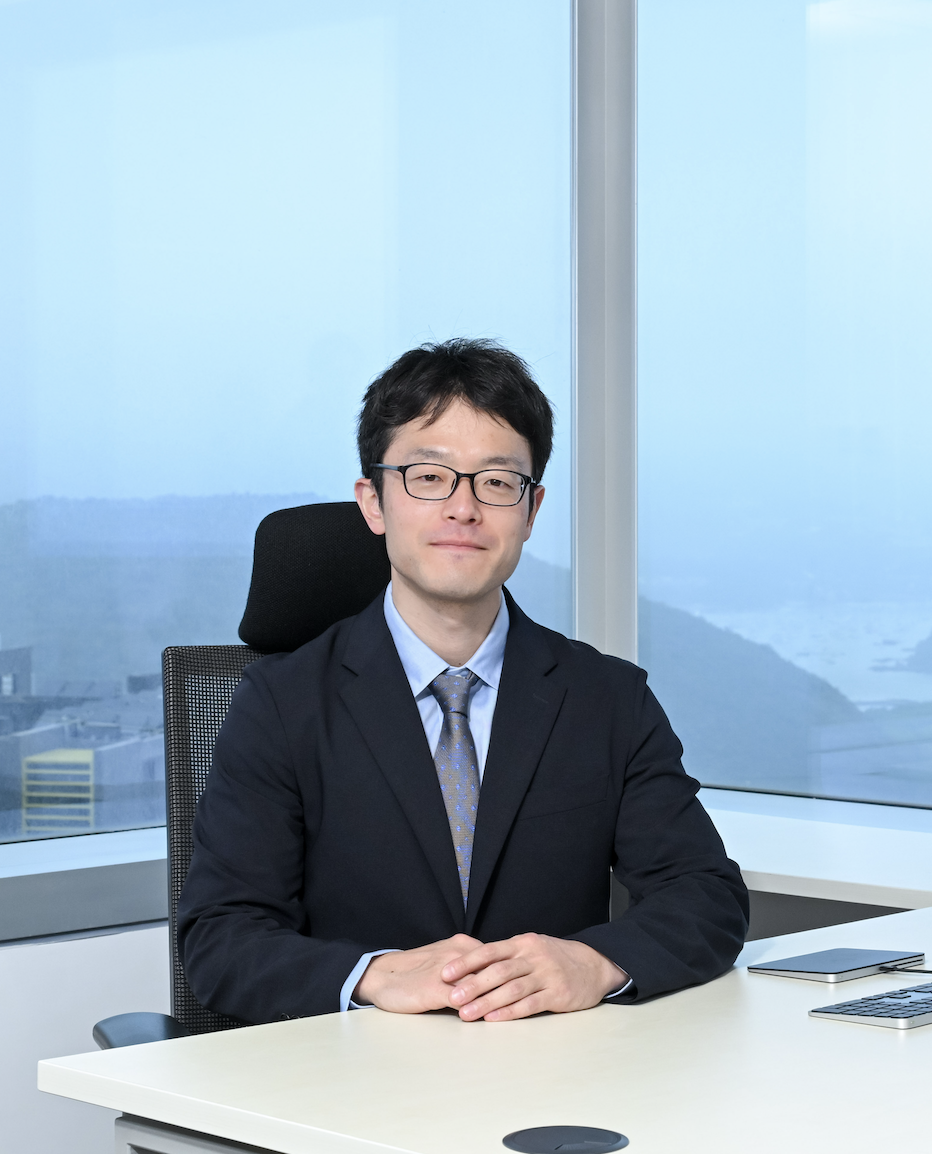
\includegraphics[width=\linewidth]{photo_cv.png}
\end{minipage}%
\hfill
\begin{minipage}[t]{0.74\textwidth}
    \vspace{0pt}
    {\huge \textbf{Haruki Watanabe}}\\[0.25cm]
    Professor of Physics \& IAS Professor\\
    Department of Physics\\
    HKUST Jockey Club Institute for Advanced Study\\
    Hong Kong University of Science and Technology\\[0.15cm]
    \begin{tabular}{@{}ll@{}}
    Office: & Room 4453, HKUST, Clear Water Bay, Kowloon, Hong Kong \\
    Phone:  & (852) 2358-7476 \\
    Email:  & \href{mailto:hwatanabe@ust.hk}{hwatanabe@ust.hk} \\
    ORCID:  & \href{https://orcid.org/0000-0002-8112-021X}{0000-0002-8112-021X} \\
    Web:    & \href{https://haruki-watanabe-hkust.github.io/group-site/index.html}{haruki-watanabe-hkust.github.io/group-site} (Japanese)
    \end{tabular}\\[0.1cm]
    {\small
    \href{https://physics.hkust.edu.hk/node/3704}{Physics Dept.}
    $\,\cdot\,$
    \href{https://researchportal.hkust.edu.hk/en/persons/haruki-watanabe/}{Research Portal}
    $\,\cdot\,$
    \href{https://ias.hkust.edu.hk/people/ias-members/faculty/prof-haruki-watanabe}{IAS Profile}}
\end{minipage}

\vspace{0.4cm}
\hrule
\vspace{0.3cm}

% --- Employment ---
\section*{Academic Appointments}
\begin{description}
    \item[Mar.~2026 -- Present:] \textbf{Professor of Physics}, Department of Physics, and \textbf{IAS Professor}, HKUST Jockey Club Institute for Advanced Study, Hong Kong University of Science and Technology
    \item[Jan.~2019 -- Feb.~2026:] \textbf{Associate Professor (PI)}, Department of Applied Physics, University of Tokyo
    \item[Feb.~2016 -- Dec.~2018:] \textbf{Lecturer (PI)}, Department of Applied Physics, University of Tokyo
    \item[Jul.~2015 -- Jan.~2016:] \textbf{Pappalardo Postdoctoral Fellow}, Massachusetts Institute of Technology
\end{description}

% --- Education ---
\section*{Education}
\begin{description}
    \item[Aug.~2011 -- May~2015:] \textbf{Ph.D. in Physics}, University of California, Berkeley (Advisor: Prof.~Ashvin Vishwanath)
    \item[Apr.~2010 -- Mar.~2012:] \textbf{M.Sc. in Physics}, University of Tokyo (with honors)
    \item[Apr.~2006 -- Mar.~2010:] \textbf{B.A. in Physics}, University of Tokyo (with honors)
\end{description}

% --- Research Interest ---
\section*{Research Interests}
Uncovering universal properties of quantum many-body systems from a symmetry perspective. My research spans several interconnected areas:
\begin{itemize}[noitemsep, topsep=3pt]
    \item \emph{Spontaneous symmetry breaking and Nambu--Goldstone bosons} ---
    Established a unified counting rule for Nambu--Goldstone bosons in nonrelativistic systems [\href{https://doi.org/10.1103/PhysRevLett.108.251602}{PRL {\bf 108}, 251602 (2012)}; \href{https://doi.org/10.1103/PhysRevX.4.031057}{PRX {\bf 4}, 031057 (2014)}], and proved the absence of quantum time crystals [\href{https://doi.org/10.1103/PhysRevLett.114.251603}{PRL {\bf 114}, 251603 (2015)}].

    \item \emph{Topological phases and symmetry indicators} ---
    Developed a symmetry-based framework for diagnosing band topology in all 230 (and 1651 magnetic) space groups [\href{https://doi.org/10.1038/s41467-017-00133-2}{Nat.~Commun.~{\bf 8}, 50 (2017)}; \href{https://doi.org/10.1126/sciadv.aat8685}{Sci.~Adv.~{\bf 4}, eaat8685 (2018)}], extended to topological superconductors [\href{https://doi.org/10.1126/sciadv.aaz8367}{Sci.~Adv.~{\bf 6}, eaaz8367 (2020)}].

    \item \emph{Nonlinear electromagnetic responses in superconductors} ---
    Formulated gauge-invariant theory of optical responses and established rigorous sum rules for nonlinear conductivities [\href{https://doi.org/10.1103/PhysRevB.102.165137}{PRB {\bf 102}, 165137 (2020)}].

    \item \emph{Frustration-free quantum many-body systems} ---
    Proved rigorous bounds on dynamical critical exponents and finite-size gaps in gapless frustration-free systems [\href{https://doi.org/10.1103/d4c4-5p2r}{PRX {\bf 15}, 041050 (2025)}; \href{https://doi.org/10.1103/PhysRevLett.133.176001}{PRL {\bf 133}, 176001 (2024)}].
\end{itemize}

% --- Awards ---
\section*{Selected Awards}
\begin{itemize}[noitemsep, topsep=3pt]
    \item \href{https://www.ap.t.u-tokyo.ac.jp/info/press/entry-680.html}{Particle Physics Medal (Japan Particle and Nuclear Theory Forum, 2025)}
    \item \href{https://www.t.u-tokyo.ac.jp/en/topics/tp2025-04-04-003}{Faculty of Engineering Best Teaching Award (University of Tokyo, 2024)}
    \item \href{https://www.mext.go.jp/b_menu/houdou/mext_01364.html}{The Commendation for Science and Technology (Minister of Education, Japan, 2024)}
    \item \href{https://breakthroughprize.org/Laureates/1/L3904}{\textbf{New Horizons in Physics Prize} (Breakthrough Prize Foundation, 2022)}
    \item \href{https://cmsp.phys.s.u-tokyo.ac.jp/en/condensed-matter-science-prize/}{Condensed-Matter Science Prize (2017)}
    \item \href{https://w.wiki/Dm9T}{Yukawa Memorial Prize (2016)}
    \item \href{http://www.r8.div.jps.or.jp/past_young_scientist_award.html}{Young Scientist Award (Physical Society of Japan, 2016)}
    \item \href{https://www2.yukawa.kyoto-u.ac.jp/~soryushi.shogakukai/jusho.html}{Seitaro Nakamura Prize (2013)}
    \item \href{https://gsi.berkeley.edu/programs-services/award-programs/ogsi/ogsi-2012/}{Outstanding Graduate Student Instructor (UC Berkeley, 2012)}
\end{itemize}

% --- Publications Summary ---
\section*{Publications}
Over 60 refereed publications (see attached publication list), including 14 in Physical Review Letters, 5 in Physical Review X, 3 in Science Advances, 2 in Proceedings of the National Academy of Sciences, and 1 in Nature Communications.
Seven papers selected as Editors' Suggestions. Author of an invited review article in Annual Review of Condensed Matter Physics [{\bf 11}, 169 (2020)].

\medskip
\noindent\textbf{Selected Publications} {\small (asterisk denotes corresponding author; underline denotes myself)}

\begin{enumerate}[noitemsep, topsep=3pt, leftmargin=2em, label={[\arabic*]}]

\item R.~Masaoka, T.~Soejima, and \underline{H.~Watanabe}*,
\emph{Rigorous lower bound of dynamic critical exponents in critical frustration-free systems,}
\href{https://doi.org/10.1103/d4c4-5p2r}{Phys.\ Rev.\ X {\bf 15}, 041050 (2025)}.

\item \underline{H.~Watanabe}*, H.~Katsura, and J.~Y.~Lee,
\emph{Critical Spontaneous breaking of U(1) symmetry at zero temperature in one dimension,}
\href{https://doi.org/10.1103/PhysRevLett.133.176001}{Phys.\ Rev.\ Lett.\ {\bf 133}, 176001 (2024)}. {\small \textcolor{red}{Editors' Suggestion}}

\item F.~Tang, S.~Ono, X.-G.~Wan, and \underline{H.~Watanabe}*,
\emph{High-throughput Investigations of Topological and Nodal Superconductors,}
\href{https://doi.org/10.1103/PhysRevLett.129.027001}{Phys.\ Rev.\ Lett.\ {\bf 129}, 027001 (2022)}. {\small \textcolor{red}{Editors' Suggestion}}

\item \underline{H.~Watanabe} and H.~C.~Po*,
\emph{Fractional Corner Charge of Sodium Chloride,}
\href{https://doi.org/10.1103/PhysRevX.11.041064}{Phys.\ Rev.\ X {\bf 11}, 041064 (2021)}.

\item S.~Ono, H.~C.~Po, and \underline{H.~Watanabe}*,
\emph{Refined symmetry indicators for topological superconductors in all space groups,}
\href{https://doi.org/10.1126/sciadv.aaz8367}{Sci.\ Adv.\ {\bf 6}, eaaz8367 (2020)}.

\item H.~C.~Po, \underline{H.~Watanabe}, and A.~Vishwanath*,
\emph{Fragile Topology and Wannier Obstructions,}
\href{https://doi.org/10.1103/PhysRevLett.121.126402}{Phys.\ Rev.\ Lett.\ {\bf 121}, 126402 (2018)}. {\small \textcolor{red}{Editors' Suggestion}}

\item E.~Khalaf, H.~C.~Po, A.~Vishwanath, and \underline{H.~Watanabe}*,
\emph{Symmetry indicators and anomalous surface states of topological crystalline insulators,}
\href{https://doi.org/10.1103/PhysRevX.8.031070}{Phys.\ Rev.\ X {\bf 8}, 031070 (2018)}.

\item \underline{H.~Watanabe} and M.~Oshikawa*,
\emph{Inequivalent Berry phases for the bulk polarization,}
\href{https://doi.org/10.1103/PhysRevX.8.021065}{Phys.\ Rev.\ X {\bf 8}, 021065 (2018)}.

\item H.~C.~Po, A.~Vishwanath*, and \underline{H.~Watanabe},
\emph{Symmetry-based indicators of band topology in the 230 space groups,}
\href{https://doi.org/10.1038/s41467-017-00133-2}{Nat.\ Commun.\ {\bf 8}, 50 (2017)}.

\item \underline{H.~Watanabe} and M.~Oshikawa*,
\emph{Absence of Quantum Time Crystals,}
\href{https://doi.org/10.1103/PhysRevLett.114.251603}{Phys.\ Rev.\ Lett.\ {\bf 114}, 251603 (2015)}.

\item \underline{H.~Watanabe} and H.~Murayama*,
\emph{Effective Lagrangian for Nonrelativistic Systems,}
\href{https://doi.org/10.1103/PhysRevX.4.031057}{Phys.\ Rev.\ X {\bf 4}, 031057 (2014)}.

\item \underline{H.~Watanabe} and H.~Murayama*,
\emph{Unified Description of Nambu--Goldstone Bosons without Lorentz Invariance,}
\href{https://doi.org/10.1103/PhysRevLett.108.251602}{Phys.\ Rev.\ Lett.\ {\bf 108}, 251602 (2012)}. {\small \textcolor{red}{Editors' Suggestion}}

\end{enumerate}

% --- Invited Talks ---
\section*{Invited Talks}
Over 40 invited talks at international workshops and conferences, including Aspen Center for Physics, ICTS Bangalore, Kavli IPMU, Kavli ITS Beijing, OIST, and UC Berkeley.  Three colloquium talks, including at Caltech.

\medskip
\noindent\textbf{Recent Invited Talks (selected)}
\begin{itemize}[noitemsep, topsep=3pt]
\item International Workshop on Quantum Geometry, RIKEN (Feb.\ 2026)
\item Generalised Symmetries and Anomalies in Quantum Phases of Matter, ICTS Bangalore (Jan.\ 2026)
\item Mathematical Foundations of Topological Materials, IAS HKUST (Jan.\ 2026)
\item 100 Years of Quantum Physics, ICISE Quy Nhon (Oct.\ 2025)
\item Aspects of Generalized Symmetries, OIST (Jun.\ 2025)
\item Unraveling the Particle World and the Cosmos, UC Berkeley (Sep.\ 2024)
\item Recent Developments and Challenges in Topological Phases, YITP Kyoto (Jun.\ 2024)
\end{itemize}

% --- Research Grants ---
\section*{Research Grants}
\begin{itemize}[noitemsep, topsep=3pt]
    \item \textbf{JSPS Grant-in-Aid for Scientific Research (B)}, \underline{US\$123.9k} (2024 -- 2028)
    \item \textbf{JSPS Grant-in-Aid for Scientific Research (B)}, \underline{US\$115.3k} (2021 -- 2024) *Co-Investigator
    \item \textbf{JSPS Grant-in-Aid for Scientific Research (B)}, \underline{US\$107.5k} (2020 -- 2024)
    \item \textbf{Japan Science and Technology PRESTO}, \underline{US\$200k} (2018 -- 2021)
    \item \textbf{JSPS Grant-in-Aid for Young Scientists (B)}, \underline{US\$27.7k} (2017 -- 2019)
    \item \textbf{Grant for the University of Tokyo Excellent Young Researchers}, \underline{US\$40k} (2017 -- 2018)
\end{itemize}
{\footnotesize (Currency conversion assumes approx. $1\,\mathrm{USD} = 150\,\mathrm{JPY}$)}

% --- Organized Workshops ---
\section*{(Co-)Organized Workshops}
\begin{itemize}[noitemsep, topsep=3pt]
    \item \textbf{Topology, Entanglement, and Dynamics in Quantum Many-Body Systems},
    Dec.\ 2025, ISSP Kashiwa\\
    \url{http://www.phys.keio.ac.jp/members/furukawa/2025topoent/}
    \item \textbf{Recent Developments on Multipole Moments in Quantum Systems},
    May 2020, via Zoom\\
    \url{https://sites.google.com/g.ecc.u-tokyo.ac.jp/workshop-multipole/}
    \item \textbf{Symmetry and Topology in Condensed-Matter Physics},
    Jun.\ 2018, University of Tokyo\\
    \url{https://sites.google.com/site/symmetrytopologycmp/}
\end{itemize}

%%%%%%%%%%%%%%%%%%%%%%%%%%%%%%%%%%%%%%%%%%%%%%%%%%%%%%%%%%%%%%
\clearpage
%%%%%%%%%%%%%%%%%%%%%%%%%%%%%%%%%%%%%%%%%%%%%%%%%%%%%%%%%%%%%%

\begin{center}
    {\Large \textbf{Full List of Publications and Talks}}\\[0.15cm]
    {\large Haruki Watanabe}
\end{center}

\vspace{0.3cm}

\begin{enumerate}

\section*{Preprints}

\item S. Watanabe, Y. Motome, \underline{H. Watanabe}*, \\\emph{Monte Carlo Study of the Phase Transition of the $XY$ Model on a Diamond Lattice.}\\{\href{https://arxiv.org/abs/2604.17939}{arXiv:2604.17939}.}

\item S. Watanabe, Y. Motome, \underline{H. Watanabe}*, \\\emph{Topological Phase Transitions and Their Thermodynamic Fate in Arbitrary-$S$ Pyrochlore Spin Ice.}\\{\href{https://arxiv.org/abs/2604.04346}{arXiv:2604.04346}.}

\item S. Watanabe, Y. Motome, \underline{H. Watanabe}*, \\\emph{Continuous crossover between high-pressure ice phases VII and X driven by monopole screening: a model study.}\\{\href{https://arxiv.org/abs/2603.19620}{arXiv:2603.19620}.}

\item S. Watanabe, Y. Motome, \underline{H. Watanabe}*, \\\emph{Dualities and Topological Classification of the $S=1$ Pyrochlore Spin Ice.}\\{\href{https://arxiv.org/abs/2603.03852}{arXiv:2603.03852}.}

\item S. Watanabe, \underline{H. Watanabe}*, \\\emph{Gauge-invariant electromagnetic responses in superconductors.}\\{\href{https://arxiv.org/abs/2501.13722}{arXiv:2501.13722}.}

\item C.-g. Oh, \underline{H. Watanabe}, N. Tsuji*, \\\emph{Role of Quantum Geometry in the Competition between Higgs Mode and Quasiparticles in Third-Harmonic Generation of Superconductors.}\\{\href{https://arxiv.org/abs/2512.01200}{arXiv:2512.01200}.}

\item S. Watanabe, \underline{H. Watanabe}*, \\\emph{A gauge-invariant formulation of optical responses in superconductors.}\\{\href{https://arxiv.org/abs/2410.18679}{arXiv:2410.18679}.}

\clearpage


\setcounter{enumi}{0}
\section*{Refereed Papers}

\item S. Ono, R. Masaoka, \underline{H. Watanabe}, H. C. Po*, \\\emph{Frustration-free free fermions.}\\{\href{https://arxiv.org/abs/2503.14312}{arXiv:2503.14312}. To appear in Phys. Rev. Research.}

\item R. Masaoka, S. Ono, H. C. Po, \underline{H. Watanabe}*, \\\emph{Frustration-free free fermions and beyond.}\\{\href{https://arxiv.org/abs/2503.12879}{arXiv:2503.12879}. To appear in Phys. Rev. B.}

\item R. Kobayashi, \underline{H. Watanabe}*, \\\emph{Projective Representations, Bogomolov Multiplier, and Their Applications in Physics.}\\{\href{https://doi.org/10.1007/s10773-025-06215-y}{International Journal of Theoretical Physics {\bf 65}, 65 (2026)}.}

\item R. Masaoka, T. Soejima, \underline{H. Watanabe}*, \\\emph{Rigorous lower bound of dynamic critical exponents in critical frustration-free systems.}\\{\href{https://doi.org/10.1103/d4c4-5p2r}{Physical Review X {\bf 15}, 041050 (2025)}.}

\item C. Lee, Y. Hu, G. Y. Cho, \underline{H. Watanabe}*, \\\emph{$\mathbb{Z}_N$ generalizations of three-dimensional stabilizer codes.}\\{\href{https://doi.org/10.1103/qctl-hwvh}{Physical Review B {\bf 112}, 155136 (2025)}. \emph{\small \textcolor{red}{Editors' Suggestion}}}

\item S. Sengoku, H. C. Po, \underline{H. Watanabe}*, \\\emph{Quasi-local Frustration-Free Free Fermions.}\\{\href{https://doi.org/10.1103/794x-jdn7}{Physical Review B {\bf 112}, 115104 (2025)}.}

\item R. Masaoka, T. Soejima, \underline{H. Watanabe}*, \\\emph{Rigorous lower bound of the dynamical critical exponent of the Ising model.}\\{\href{https://doi.org/10.1007/s10955-025-03456-3}{Journal of Statistical Physics {\bf 192}, 76 (2025)}.}

\item R. Masaoka, T. Soejima, \underline{H. Watanabe}*, \\\emph{Quadratic dispersion relations in gapless frustration-free systems.}\\{\href{https://doi.org/10.1103/PhysRevB.110.195140}{Physical Review B {\bf 110}, 195140 (2024)}.}

\item \underline{H. Watanabe}, H. Katsura, and J. Y. Lee*, \\\emph{Critical Spontaneous breaking of U(1) symmetry at zero temperature in one dimension.}\\{\href{https://doi.org/10.1103/PhysRevLett.133.176001}{Physical Review Letters {\bf 133}, 176001 (2024)}. \emph{\small \textcolor{red}{Editors' Suggestion}}}

\item S. Ono, K. Shiozaki, and \underline{H. Watanabe}*, \\\emph{Classification of time-reversal symmetric topological superconducting phases for conventional pairing symmetries.}\\{\href{https://doi.org/10.1103/PhysRevB.109.214502}{Physical Review B {\bf 109}, 214502 (2024)}.}

\item C. Oh and \underline{H. Watanabe}*, \\\emph{Revisiting electromagnetic response of superconductors in mean-field approximation.}\\{\href{https://doi.org/10.1103/PhysRevResearch.6.013058}{Physical Review Research {\bf 6}, 013058 (2024)}.}

\item Y. Hu and  \underline{H. Watanabe}*, \\\emph{Spontaneous symmetry breaking without ground state degeneracy in generalized $N$-state clock model.}\\{\href{https://doi.org/10.1103/PhysRevB.107.195139}{Physical Review B {\bf 107}, 195139 (2023)}.}

\item \underline{H. Watanabe}, M. Cheng, and Y. Fuji*, \\\emph{Ground state degeneracy on torus in a family of $\mathbb{Z}_N$ toric code.}\\{\href{https://doi.org/10.1063/5.0134010}{Journal of Mathematical Physics {\bf 64}, 051901 (2023)}.}

\item K. Takasan, M. Oshikawa, and \underline{H. Watanabe}*, \\\emph{Drude weights in one-dimensional systems with a single defect.}\\{\href{https://doi.org/10.1103/PhysRevB.107.075141}{Physical Review B {\bf 107}, 075141 (2023)}.}

\item H. Kobayashi and \underline{H. Watanabe}*, \\\emph{Vanishing and nonvanishing persistent currents of various conserved quantities.}\\{\href{https://doi.org/10.1103/PhysRevLett.129.176601}{Physical Review Letters {\bf 129}, 176601 (2022)}.}

\item F. Tang, S. Ono, X.-G. Wan, and \underline{H. Watanabe}*, \\\emph{High-throughput Investigations of Topological and Nodal Superconductors.}\\{\href{https://doi.org/10.1103/PhysRevLett.129.027001}{Physical Review Letters {\bf 129}, 027001 (2022)}. \emph{\small \textcolor{red}{Editors' Suggestion}}}

\item \underline{H. Watanabe}*, \\\emph{The Bloch theorem in the presence of an additional conserved charge.}\\{\href{https://doi.org/10.1103/PhysRevResearch.4.013043}{Physical Review Research {\bf 4}, 013043 (2022)}.}

\item K. Naito, R. Takahashi, \underline{H. Watanabe}, and S. Murakami*, \\\emph{Fractional hinge and corner charges in various crystal shapes with cubic symmetry.}\\{\href{https://doi.org/10.1103/PhysRevB.105.045126}{Physical Review B {\bf 105}, 045126 (2022)}.}

\item Y. Liu, Y. Fuji, and \underline{H. Watanabe}*, \\\emph{Bloch oscillations in the spin-1/2 XXZ chain.}\\{\href{https://doi.org/10.1103/PhysRevB.104.205115}{Physical Review B {\bf 104}, 205115 (2021)}.}

\item H. Tasaki and \underline{H. Watanabe}*, \\\emph{Off-Diagonal Long-Range Order Implies Vanishing Charge Gap.}\\{\href{https://doi.org/10.1103/PhysRevB.104.L180501}{Physical Review B {\bf 104}, L180501 (2021)}.}

\item \underline{H. Watanabe} and H. C. Po*, \\\emph{Fractional Corner Charge of Sodium Chloride.}\\{\href{https://doi.org/10.1103/PhysRevX.11.041064}{Physical Review X {\bf 11}, 041064 (2021)}.}

\item  \underline{H. Watanabe}, Y. Kato, H. C. Po, and Y. Motome*, \\\emph{Fractional corner magnetization of collinear antiferromagnets.}\\{\href{https://doi.org/10.1103/PhysRevB.103.134430}{Physical Review B {\bf 103}, 134430 (2021)}.}

\item A. Matsugatani, S. Ono, Y. Nomura, and \underline{H. Watanabe}*, \\\emph{qeirreps: an open-source program for Quantum ESPRESSO to compute irreducible representations of Bloch wavefunctions.}\\{\href{https://doi.org/10.1016/j.cpc.2021.107948}{Computer Physics Communications {\bf 264}, 107948 (2021)}.}

\item \underline{H. Watanabe}, Y. Liu, and M. Oshikawa*, \\\emph{On the general properties of non-linear optical conductivities.}\\{\href{https://doi.org/10.1007/s10955-020-02654-5}{Journal of Statistical Physics {\bf 181}, 2050 (2020)}.}

\item \underline{H. Watanabe} and M. Oshikawa*, \\\emph{Generalized $f$-Sum Rules and Kohn formulas on Non-linear Conductivities.}\\{\href{https://doi.org/10.1103/PhysRevB.102.165137}{Physical Review B {\bf 102}, 165137 (2020)}.}

\item \underline{H. Watanabe} and S. Ono*, \\\emph{Corner charge and bulk multipole moment in periodic systems.}\\{\href{https://doi.org/10.1103/PhysRevB.102.165120}{Physical Review B {\bf 102}, 165120 (2020)}.}

\item S. Ono, H. C. Po, and \underline{H. Watanabe}*, \\\emph{Refined symmetry indicators for topological superconductors in all space groups.}\\{\href{https://doi.org/10.1126/sciadv.aaz8367}{Science Advances {\bf 6}, eaaz8367 (2020)}.}

\item \underline{H. Watanabe}, M. Oshikawa,  and T. Koma*, \\\emph{Proof of the absence of long-range temporal orders in Gibbs states.}\\{\href{https://doi.org/10.1007/s10955-019-02471-5}{Journal of Statistical Physics {\bf 178}, 926 (2020)}.}

\item S. Ono, L. Trifunovic, and \underline{H. Watanabe}*, \\\emph{Difficulties in operator-based formulation of the bulk quadrupole moment.}\\{\href{https://doi.org/10.1103/PhysRevB.100.245133}{Physical Review B {\bf 100}, 245133 (2019)}.}

\item \underline{H. Watanabe}*, \\\emph{A proof of the Bloch theorem for lattice models.}\\{\href{https://doi.org/10.1007/s10955-019-02386-1}{Journal of Statistical Physics {\bf 177}, 717 (2019)}.}

\item L. Trifunovic, S. Ono, and \underline{H. Watanabe}*, \\\emph{Geometric orbital magnetization in adiabatic processes.}\\{\href{https://doi.org/10.1103/PhysRevB.100.054408}{Physical Review B {\bf 100}, 054408 (2019)}.}

\item S. Ono, Y. Yanase, and \underline{H. Watanabe}*, \\\emph{Symmetry indicators for topological superconductors.}\\{\href{https://doi.org/10.1103/PhysRevResearch.1.013012}{Physical Review Research {\bf 1}, 013012 (2019)}.}

\item K. Kudo, \underline{H. Watanabe}, T. Kariyado, and Y. Hatsugai*, \\\emph{Many-body Chern number without integration.}\\{\href{https://doi.org/10.1103/PhysRevLett.122.146601}{Physical Review Letters {\bf 122}, 146601 (2019)}. \emph{\small \textcolor{red}{Editors' Suggestion}}}

\item D. V. Else, H. C. Po, and \underline{H. Watanabe}*, \\\emph{Fragile topological phases in interacting systems.}\\{\href{https://doi.org/10.1103/PhysRevB.99.125122}{Physical Review B {\bf 99}, 125122 (2019)}.}

\item \underline{H. Watanabe} and L. Lu*, \\\emph{Space-group theory of photonic crystals.}\\{\href{https://doi.org/10.1103/PhysRevLett.121.263903}{Physical Review Letters {\bf 121}, 263903 (2018)}.}

\item A. Matsugatani and \underline{H. Watanabe}*, \\\emph{Connecting higher-order topological insulators to lower-dimensional topological insulators.}\\{\href{https://doi.org/10.1103/PhysRevB.98.205129}{Physical Review B {\bf 98}, 205129 (2018)}.}

\item \underline{H. Watanabe}*, \\\emph{Insensitivity of bulk properties to the twisted boundary condition.}\\{\href{https://doi.org/10.1103/PhysRevB.98.155137}{Physical Review B {\bf 98}, 155137 (2018)}.}

\item S. Ono and \underline{H. Watanabe}*, \\\emph{Unified understanding of symmetry indicators for all internal symmetry classes.}\\{\href{https://doi.org/10.1103/PhysRevB.98.115150}{Physical Review B {\bf 98}, 115150 (2018)}.}

\item E. Khalaf, H. C. Po, A. Vishwanath, and \underline{H. Watanabe}*, \\\emph{Symmetry indicators and anomalous surface states of topological crystalline insulators.}\\{\href{https://doi.org/10.1103/PhysRevX.8.031070}{Physical Review X {\bf 8}, 031070 (2018)}.}

\item \underline{H. Watanabe} and M. Oshikawa*, \\\emph{Inequivalent Berry phases for the bulk polarization.}\\{\href{https://doi.org/10.1103/PhysRevX.8.021065}{Physical Review X {\bf 8}, 021065 (2018)}.}

\item \underline{H. Watanabe}*, \\\emph{The Lieb-Schultz-Mattis-type filling constraints in the 1651 magnetic space groups.}\\{\href{https://doi.org/10.1103/PhysRevB.97.165117}{Physical Review B {\bf 97}, 165117 (2018)}.} \emph{\small \textcolor{red}{Editors' Suggestion}}

\item A. Matsugatani, Y. Ishiguro, K. Shiozaki, and \underline{H. Watanabe}*, \\\emph{Universal Relation among the Many-Body Chern Number, Rotation Symmetry, and Filling.}\\{\href{https://doi.org/10.1103/PhysRevLett.120.096601}{Physical Review Letters {\bf 120}, 096601 (2018)}.}

\item H. C. Po, \underline{H. Watanabe}, and A. Vishwanath*, \\\emph{Fragile Topology and Wannier Obstructions.}\\{\href{https://doi.org/10.1103/PhysRevLett.121.126402}{Physical Review Letters {\bf 121}, 126402 (2018)}. \emph{\small \textcolor{red}{Editors' Suggestion}}}

\item \underline{H. Watanabe}, H. C. Po, and A. Vishwanath*, \\\emph{Structure and Topology of Band Structures in the 1651 Magnetic Space Groups.}\\{\href{https://doi.org/10.1126/sciadv.aat8685}{Science Advances {\bf 4}, eaat8685 (2018)}.}


\item H. C. Po, \underline{H. Watanabe}, C.-M. Jian, and  M. P. Zaletel*, \\\emph{Lattice Homotopy Constraints on Phases of Quantum Magnets.}\\{\href{https://doi.org/10.1103/PhysRevLett.119.127202}{Physical Review Letters {\bf 119}, 127202 (2017)}.}

\item H. C. Po, A. Vishwanath*, and \underline{H. Watanabe}, \\\emph{Symmetry-based indicators of band topology in the 230 space groups.}\\{\href{https://doi.org/10.1038/s41467-017-00133-2}{Nature Communications {\bf 8}, 50 (2017)}.}

\item \underline{H. Watanabe} and L. Fu*, \\\emph{Topological crystalline magnets: Symmetry-protected topological phases of fermions.}\\{\href{https://doi.org/10.1103/PhysRevB.95.081107}{Physical Review B (Rapid Communications) {\bf 95}, 081107 (2017)}.}

\item \underline{H. Watanabe}*, \\\emph{Energy Gap of Neutral Excitations Implies Vanishing Charge Susceptibility.}\\{\href{https://doi.org/10.1103/PhysRevLett.118.117205}{Physical Review Letters {\bf 118}, 117205 (2017)}.}

\item \underline{H. Watanabe}, H. C. Po, M. P. Zaletel, and A. Vishwanath*, \\\emph{Filling-Enforced Gaplessness in Band Structures of the 230 Space Groups.}\\{\href{https://doi.org/10.1103/PhysRevLett.117.096404}{Physical Review Letters {\bf 117}, 096404 (2016)}.}

\item H. C. Po, \underline{H. Watanabe}, M. P. Zaletel, and A. Vishwanath*, \\\emph{Filling-enforced quantum band insulators in spin-orbit coupled crystals.}\\{\href{https://doi.org/10.1126/sciadv.1501782}{Science Advances {\bf 2}, e1501782 (2016)}.}

\item \underline{H. Watanabe} and A. Vishwanath*, \\\emph{Electric Field-Induced Skyrmion Crystals via Charged Monopoles in Insulating Helimagets.}\\{\href{https://doi.org/10.7566/JPSJ.85.064707}{Journal of the Physical Society of Japan {\bf 85}, 064707 (2016)}.}


\item \underline{H. Watanabe}, H. C. Po, A. Vishwanath, and M. P. Zaletel*, \\\emph{Filling constraints for spin-orbit coupled insulators in symmorphic and nonsymmorphic crystals.}\\{\href{https://doi.org/10.1073/pnas.1514665112}{Proceedings of the National Academy of Science {\bf 112}, 14551 (2015)}.}

\item \underline{H. Watanabe} and M. Oshikawa*, \\\emph{Absence of Quantum Time Crystals.}\\{\href{https://doi.org/10.1103/PhysRevLett.114.251603}{Physical Review Letters {\bf 114}, 251603 (2015)}.}

\item \underline{H. Watanabe} and H. Murayama*, \\\emph{Spontaneously broken non-Abelian gauge symmetries in nonrelativistic systems.}\\{\href{https://doi.org/10.1103/PhysRevD.90.121703}{Physical Review D (Rapid Communications) {\bf 90}, 121703 (2014)}.}

\item \underline{H. Watanabe} and A. Vishwanath*, \\\emph{Criterion for stability of Goldstone modes and Fermi liquid behavior in a metal with broken symmetry.}\\{\href{https://doi.org/10.1073/pnas.1415592111}{Proceedings of the National Academy of Science {\bf 111}, 16314 (2014)}.}

\item \underline{H. Watanabe} and H. Murayama*, \\\emph{Nambu-Goldstone bosons with fractional-power dispersion relations.}\\{\href{https://doi.org/10.1103/PhysRevD.89.101701}{Physical Review D (Rapid Communications) {\bf 89}, 101701 (2014)}.}

\item \underline{H. Watanabe} and H. Murayama*, \\\emph{Effective Lagrangian for Nonrelativistic Systems.}\\{\href{https://doi.org/10.1103/PhysRevX.4.031057}{Physical Review X {\bf 4}, 031057 (2014)}.}

\item \underline{H. Watanabe} and H. Murayama*, \\\emph{Noncommuting Momenta of Topological Solitons.}\\{\href{https://doi.org/10.1103/PhysRevLett.112.191804}{Physical Review Letters {\bf 112}, 191804 (2014)}.}

\item T. Brauner and \underline{H. Watanabe}*, \\\emph{Spontaneous breaking of spacetime symmetries and the inverse Higgs effect.}\\{\href{https://doi.org/10.1103/PhysRevD.89.085004}{Physical Review D {\bf 89}, 085004 (2014)}.}

\item \underline{H. Watanabe}, S. A. Parameswaran, S. Raghu, and A. Vishwanath*, \\\emph{Anomalous Fermi-liquid phase in metallic skyrmion crystals.}\\{\href{https://doi.org/10.1103/PhysRevB.90.045145}{Physical Review B {\bf 90}, 045145 (2014)}.}

\item \underline{H. Watanabe}, T. Brauner, and H. Murayama*, \\\emph{Massive Nambu-Goldstone Bosons.}\\{\href{https://doi.org/10.1103/PhysRevLett.111.021601}{Physical Review Letters {\bf 111}, 021601 (2013)}.}

\item \underline{H. Watanabe} and H. Murayama*, \\\emph{Redundancies in Nambu-Goldstone Bosons.}\\{\href{https://doi.org/10.1103/PhysRevLett.110.181601}{Physical Review Letters {\bf 110}, 181601 (2013)}.}

\item \underline{H. Watanabe} and H. Murayama*, \\\emph{Unified Description of Nambu-Goldstone Bosons without Lorentz Invariance.}\\{\href{https://doi.org/10.1103/PhysRevLett.108.251602}{Physical Review Letters {\bf 108}, 251602 (2012)}.} \emph{\small \textcolor{red}{Editors' Suggestion; highlighted in Physics Synopsis (Physics 5, s93).}}


\item \underline{H. Watanabe} and T. Brauner*, \\\emph{Spontaneous breaking of continuous translational invariance.}\\{\href{https://doi.org/10.1103/PhysRevD.85.085010}{Physical Review D {\bf 85}, 085010 (2012)}.}

\item \underline{H. Watanabe} and T. Brauner*, \\\emph{Number of Nambu-Goldstone bosons and its relation to charge densities.}\\{\href{https://doi.org/10.1103/PhysRevD.84.125013}{Physical Review D {\bf 84}, 125013 (2011)}.}

\item \underline{H. Watanabe}, Y. Hatsugai, and H. Aoki*, \\\emph{Half-integer contributions to the quantum Hall conductivity from single Dirac cones.}\\{\href{https://doi.org/10.1103/PhysRevB.82.241403}{Physical Review B (Rapid Communications) {\bf 82}, 241403 (2010)}.}

\setcounter{enumi}{0}
\section*{Review}
\item \underline{H. Watanabe}*, \\\emph{Counting Rules of Nambu-Goldstone Modes.}\\
{\href{https://doi.org/10.1146/annurev-conmatphys-031119-050644}{Annual Review of Condensed Matter Physics {\bf 11}, 169 (2020)}.}

\setcounter{enumi}{0}
\section*{Proceedings}

\item \underline{H. Watanabe}, Y. Hatsugai, and H. Aoki*, \\\emph{Manipulation of the Dirac cones and the anomaly in the graphene related quantum Hall effect.}\\{\href{https://doi.org/10.1088/1742-6596/334/1/012044}{Journal of Physics: Conference Series {\bf 334}, 012044 (2011)}.}



\setcounter{enumi}{0}
\section*{Invited Talks in International Workshops / Conferences}

\item International Workshop on Quantum Geometry\\
Feb. 3 -- Feb. 6  (2026) RIKEN (Wako, Japan)\\
\emph{General Properties of Frustration-Free Quantum Many-Body Systems.}

\item New Frontiers of Geometry and Topology in Condensed Matter Physics\\
Jan. 26 -- Feb. 9  (2026) ISSP (Kashiwa, Japan)\\
\emph{General Properties of Frustration-Free Quantum  Many-Body Systems.}

\item Generalised symmetries and anomalies in quantum phases of matter\\
Jan. 5 -- Jan. 16  (2026) ICTS (Bangalore, India)\\
\emph{Frustration-Free Quantum Many-Body Systems.}

\item Mathematical Foundations of Topological Materials\\
Jan. 6 -- Jan. 9  (2026) IAS, HKUST (Hong Kong)\\
\emph{General Properties of Frustration-Free Systems.}

\item Topology, Entanglement, and Dynamics
in Quantum Many-Body Systems\\
Dec. 22  (2025) ISSP (Kashiwa, Japan)\\
\emph{Frustration-Free Quantum Many-Body Systems.}

\item 100 Years of Quantum Physics\\
Oct. 6 -- Oct. 9 (2025) International Centre for Interdisciplinary Science and Education (Quy Nhon, Vietnam)\\
\emph{General Properties of Frustration-Free Quantum Many-Body Systems.}

\item Frontiers of Quantum Matter\\
Aug. 14 -- Aug. 6 (2025) Longfu Cultural Center (Beijing, China)\\
\emph{General Properties of Frustration-Free Quantum Many-Body Systems.}

\item Aspects of Generalized Symmetries\\
Jun. 16 -- Jun. 20 (2025) OIST (Okinawa, Japan)\\
\emph{General properties of frustration-free systems.}

\item Frontiers in Field Theory and Phenomenology\\
May 19 -- May 23 (2025) Kavli IPMU (Kashiwa, Japan)\\
\emph{Conjectures on frustration free systems.}

\item Phases of Matter from an Informational Perspective\\
Dec. 4 -- Dec. 11 (2024) Hong Kong University of Science and Technology (Hong Kong)\\
\emph{Finite size gaps and low-energy excitations in gapless frustration free systems.}

\item Effective Field Theory Beyond Ordinary Symmetries\\
Dec. 2 -- Dec. 6 (2024) Institute for Basic Science (Daejeon, Korea)\\
\emph{Finite size gaps and low-energy excitations in gapless frustration free systems.}

\item Unraveling the Particle World and the Cosmos at Berkeley\\
Sep. 26 -- Sep. 28 (2024) UC Berkeley (Berkeley, USA)\\
\emph{Finite size gaps and low-energy excitations in gapless frustration free systems.}

\item Recent Developments and Challenges in Topological Phases\\
Jun. 3 -- Jun. 14 (2024) Yukawa Institute for Theoretical Physics (Kyoto, Japan)\\
\emph{Finite size gaps and low-energy excitations in gapless frustration free systems.}

\item Condensed Matter Physics Conference 2023\\
Aug. 7 -- Aug. 11 (2023) Yangtze River Delta Physics Research Center (Liyang, China)\\
\emph{Spin models for spontaneous symmetry breaking, topological orders, and fractons with weird ground state degeneracy.}

\item Theoretical studies of topological phases of matter\\
Apr. 4 -- Apr. 6 (2023) International Institute for Advanced Studies (Kyoto, Japan)\\
\emph{Ground state degeneracy on torus in topologically ordered phases and in symmetry-broken phases.}

\item Topological Phases of Matter: From Low to High Energy\\
Mar. 6 -- Mar. 10 (2023) Institute of Nuclear Theory (Seattle, USA)\\
\emph{Ground state degeneracy on torus in topologically ordered phases and in symmetry-broken phases.}

\item Novel Quantum States in Condensed Matter 2022\\
Oct. 31 -- Dec. 2 (2022) Yukawa Institute for Theoretical Physics (Kyoto, Japan)\\
\emph{Ground state degeneracy on torus in topologically ordered phases.}

\item Advances in The Physics of Topological and Correlated Matter\\
Sep. 19 -- Sep. 23 (2022) Institute for Basic Science (Dejeon, Korea)\\
\emph{Topological Material Search via Symmetry Indicator and Filling Anomaly.}

\item Topological Quantum Electrons Interacting In-person\\
July 10 -- July 16 (2022) International Centre for Interdisciplinary Science and Education (Quy Nhon, Vietnam)\\
\emph{Vanishing and nonvanishing persistent currents of various conserved quantities.}

\item
Focus Week on Quantum Mechanical Systems at Large Quantum Number\\
Sep. 3 (2021) online (IPMU, Japan)\\
\emph{Bulk-boundary correspondence of topologically trivial insulators.}

\item
Correlated Electrons Virtual International Seminars (CEVIS)\\
Mar. 25 (2021) online\\
\emph{Multipole moments and fractional corner charges of insulating materials.}

\item
Novel Phases of Quantum Matter \\
Dec. 23 (2019) -- Jan. 2 (2020) International Centre for Theoretical Sciences (Bengaluru, India)\\
\emph{Symmetry indicators for topological superconductors.}


\item
The 5th East Asia Joint Seminars on Statistical Physics\\
Oct. 22 -- Oct. 25 (2019) Chinese Academy of Sciences (Beijing, China)\\
\emph{Quantum Quench and $f$-sum Rules on Linear and Non-Linear Conductivities.}

\item
The Future of Topological Materials\\
Oct. 2 -- Oct. 5 (2019) Princeton Univ (USA)\\
\emph{Symmetry indicators for topological superconductors.}

\item
SPICE workshop: Young Research Leaders Group Workshop\\
Sep. 30 -- Oct. 3 (2019) Johannes Gutenberg Univ (Mainz, Germany)\\
\emph{Symmetry indicators for topological superconductors.}

\item
The 2nd Workshop on Spin-orbit Coupled Topological States\\
Sep. 19 -- Sep. 21 (2019) POSTECH (Pohang, Korea)\\
\emph{Symmetry indicators for topological superconductors.}

\item Theoretical studies of topological phases of matter\\
Feb. 12 -- Feb. 15 (2019) U Tokyo (Komaba, Japan)\\
\emph{Symmetry indicators of band topology I--III.}

\item Workshop on Recent Developments in Chiral Matter and Topology\\
Dec. 6 -- Dec. 9 (2018) National Taiwan Univ (Taipei, Taiwan)\\
\emph{Symmetry-Based Indicator and Fragile Topology with/without Interactions.}

\item Topological Phases and Excitations of Quantum Matter\\
Jun. 24 -- Jul. 29 (2018) Aspen Center For Physics (Aspen, USA)\\
\emph{Symmetry-Based Indicator and Fragile Topology with/without Interactions.}

\item
Topological Phases with Higher-Order Boundary States\\
Jul. 12 -- Jul. 13 (2018) Freie Universit\"at (Berlin, Germany)\\
\emph{Symmetry-based Indicators for higher-order topological insulators.}

\item
Topological Phases of Matter: from the Quantum Hall Effect to Spin Liquids\\
Jun. 11 -- Jul. 6 (2018) Kavli Institute for Theoretical Sciences (Saclay, France)\\
\emph{Many-body polarization and Thouless pump via twisted boundary condition.}

\item
New Paradigms in Quantum Matter 2018\\
Jun. 25 -- Jul. 6 (2018) Institute of Physics, Chinese Academy of Sciences (Beijing, China)\\
\emph{Symmetry-based Indicators of Topology.}

\item
Topology and Correlation\\
Jun. 7 -- Jun. 8 (2018) Korea Institute for Advanced Study (Seoul, Korea)\\
\emph{Symmetry-based Indicators of Topology.}

\item
Novel Quantum States in Condensed Matter 2017\\
Oct. 23 -- Nov. 24 (2017) Yukawa Institute for Theoretical Physics (Kyoto, Japan)\\
\emph{Complete Theory of Symmetry-based Indicators of Band Topology.}

\item
Topological States and Phase Transitions in Strongly Correlated Systems\\
Jul. 3 -- Jul. 21 (2017) Kavli Institute for Theoretical Sciences (Beijing, China)\\
\emph{Complete Theory of Symmetry-based Indicators of Band Topology.}

\item
SPICE workshop: Spin Dynamics in the Dirac Systems\\
Jun. 7 -- Jun. 9 (2017) Schloss Waldthausen (Mainz, Germany)\\
\emph{Complete Theory of Symmetry-based Indicators of Band Topology.}

\item
Theory of Correlated Topological Materials\\
Feb. 6 -- Mar. 3 (2017) Institute for Solid State Physics (Kashiwa, Japan)\\
\emph{More on the Lieb-Schultz-Mattis theorem.}

\item
International School on Topological Science and Topological Matters\\
Feb. 13 -- Feb. 18 (2017) Yukawa Institute for Theoretical Physics (Kyoto, Japan)\\
\emph{Extensions of Lieb-Schultz-Mattis theorem and its applications to quantum spin liquid and topological semimetals.}

\item
The 2nd Conference on Condensed Matter Physics\\
Jul. 20 -- Jul. 22 (2016) Nanjing University (Nanjing, China)\\
\emph{Filling-enforced gaplessness in nonsymmorphic space groups.}

\item
Nambu and Science Frontier\\
Nov. 17 (2015) Osaka University (Osaka, Japan)\\
\emph{Nambu-Goldstone Bosons in Nonrelativistic Systems.}

\item
Higgs Modes in Condensed Matter and Quantum Gases\\
Jun. 23 -- Jun. 25 (2014) Yukawa Institute for Theoretical Physics (Kyoto, Japan)\\
\emph{Nambu-Goldstone Bosons in Nonrelativistic Systems.}

\item
Non-Fermi Liquids\\
Apr. 17 -- Apr. 18 (2014) Stanford University (California, USA)\\
\emph{Criterion for Non-Fermi Liquid Phases via Interactions with Nambu-Goldstone Bosons.}

\item
Effective Field Theories for Quantum Many-Body Systems\\
Jan. 15 -- Jan. 17 (2014) Institute for Theoretical Physics (Madrid, Spain)\\
\emph{Noncommuting Momenta and the Dynamics of Translational Moduli.}

\setcounter{enumi}{0}
\section*{Colloquium Talks}
\item
Pohang University of Science and Technology (Pohang, Korea)\\
Dec. 5 (2022)\\
\emph{New twist in familiar spin models.}

\item
Physics Colloquium at University of Tokyo (Tokyo, Japan)\\
Dec. 18 (2021) online\\
\emph{Fractional corner charges of multipole insulators.}

\item
Physics Colloquium at California Institute of Technology (Pasadena, USA)\\
Dec. 3 (2020) online\\
\emph{Multipole moments and fractional corner charges of insulating materials.}


\end{enumerate}

\end{document}
